\documentclass[
	% -- opções da classe memoir --
	12pt,				% tamanho da fonte
	oneside,			% para impressão em verso e anverso. Oposto a oneside
	a4paper,			% tamanho do papel. 
	% -- opções da classe abntex2 --
	%chapter=TITLE,		% títulos de capítulos convertidos em letras maiúsculas
	%section=TITLE,		% títulos de seções convertidos em letras maiúsculas
	%subsection=TITLE,	% títulos de subseções convertidos em letras maiúsculas
	%subsubsection=TITLE,% títulos de subsubseções convertidos em letras maiúsculas
	% -- opções do pacote babel --
	english,			% idioma adicional para hifenização
	french,				% idioma adicional para hifenização
	spanish,			% idioma adicional para hifenização
	brazil,				% o último idioma é o principal do documento
	]{abntex2}


% ---
% PACOTES
% ---

% ---
% Pacotes fundamentais 
% ---
\usepackage{cmap}				% Mapear caracteres especiais no PDF
\usepackage{lmodern}			% Usa a fonte Latin Modern			
\usepackage[T1]{fontenc}		% Selecao de codigos de fonte.
\usepackage[utf8]{inputenc}		% Codificacao do documento (conversão automática dos acentos)
\usepackage{lastpage}			% Usado pela Ficha catalográfica
\usepackage{indentfirst}		% Indenta o primeiro parágrafo de cada seção.
\usepackage{color}				% Controle das cores
\usepackage{graphicx}			% Inclusão de gráficos
\usepackage[labelfont=bf,textfont=md]{caption}
% ---
		
% ---
% Pacotes adicionais, usados apenas no âmbito do Modelo Canônico do abnteX2
% ---
\usepackage{lipsum}				% para geração de dummy text
% ---

% ---
% Pacotes de citações
% ---
\usepackage[brazilian,hyperpageref]{backref}	 % Paginas com as citações na bibl
\usepackage[alf]{abntex2cite}	% Citações padrão ABNT

% --- 
% CONFIGURAÇÕES DE PACOTES
% --- 

% ---
% Configurações do pacote backref
% Usado sem a opção hyperpageref de backref
\renewcommand{\backrefpagesname}{Citado na(s) página(s):~}
% Texto padrão antes do número das páginas
\renewcommand{\backref}{}
% Define os textos da citação
\renewcommand*{\backrefalt}[4]{
	\ifcase #1 %
		Nenhuma citação no texto.%
	\or
		Citado na página #2.%
	\else
		Citado #1 vezes nas páginas #2.%
	\fi}%
% ---


% ---
% Informações de dados para CAPA e FOLHA DE ROSTO
% ---
\titulo{TITULO DO TRABALHO}
\autor{NOME DO ALUNO}
\local{Novo Hamburgo}
\data{2018}
\orientador{ORIENTADOR}
\instituicao{UNIVERSIDADE FEEVALE}
\tipotrabalho{Tese (Doutorado)}
% O preambulo deve conter o tipo do trabalho, o objetivo, 
% o nome da instituição e a área de concentração 
\preambulo{Trabalho de Conclusão de Curso apresentado como requisito parcial à obtenção do grau de Bacharel em Ciência da Computação pela Universidade Feevale}
% ---

% ---
% Configurações de aparência do PDF final

% alterando o aspecto da cor azul
\definecolor{blue}{RGB}{41,5,195}
\definecolor{black}{RGB}{0,0,0}

% informações do PDF
\makeatletter
\hypersetup{
     	%pagebackref=true,
		pdftitle={\@title}, 
		pdfauthor={\@author},
    	pdfsubject={\imprimirpreambulo},
	    pdfcreator={LaTeX with abnTeX2},
		pdfkeywords={abnt}{latex}{abntex}{abntex2}{trabalho acadêmico}, 
		colorlinks=true,       		% false: boxed links; true: colored links
    	linkcolor=black,          	% color of internal links
    	citecolor=blue,        		% color of links to bibliography
    	filecolor=magenta,    		% color of file links
		urlcolor=blue,
		bookmarksdepth=4
}
\makeatother
% --- 

% --- 
% Espaçamentos entre linhas e parágrafos 
% --- 

% O tamanho do parágrafo é dado por:
\setlength{\parindent}{1.5cm}

% Controle do espaçamento entre um parágrafo e outro:
\setlength{\parskip}{0.2cm}  % tente também \onelineskip

% ---
% compila o indice
% ---
\makeindex
% ---

% ----
% Início do documento
% ----
\begin{document}

% Retira espaço extra obsoleto entre as frases.
\frenchspacing 

% ----------------------------------------------------------
% ELEMENTOS PRÉ-TEXTUAIS
% ----------------------------------------------------------
% \pretextual

% ---
% Capa
% ---
\imprimircapa
% ---
% ---
% Folha de rosto
% ---
\imprimirfolhaderosto
% ---

% ---
% Agradecimentos
% ---
\imprimiragradecimento{Os agradecimentos principais são direcionados a todo mundo...}

% ---

% ---

% ---
% RESUMOS
% ---

% resumo em português
\begin{resumo}
 Segundo a \citeonline[3.1-3.2]{NBR6028:2003}, o resumo deve ressaltar o
 objetivo, o método, os resultados e as conclusões do documento. A ordem e a extensão
 destes itens dependem do tipo de resumo (informativo ou indicativo) e do
 tratamento que cada item recebe no documento original. O resumo deve ser
 precedido da referência do documento, com exceção do resumo inserido no
 próprio documento. (\ldots) As palavras-chave devem figurar logo abaixo do
 resumo, antecedidas da expressão Palavras-chave:, separadas entre si por
 ponto e finalizadas também por ponto.

 \vspace{\onelineskip}
    
 \noindent
 \textbf{Palavras-chaves}: latex. abntex. editoração de texto.
\end{resumo}

% resumo em inglês
\begin{resumo}[Abstract]
 \begin{otherlanguage*}{english}
   This is the english abstract.

   \vspace{\onelineskip}
 
   \noindent 
   \textbf{Key-words}: latex. abntex. text editoration.
 \end{otherlanguage*}
\end{resumo}

% ---

% ---
% inserir lista de ilustrações
% ---
\pdfbookmark[0]{\listfigurename}{lof}
\listoffigures*
\cleardoublepage
% ---

% ---
% inserir lista de tabelas
% ---
\pdfbookmark[0]{\listtablename}{lot}
\listoftables*
\cleardoublepage
% ---

% ---
% inserir lista de abreviaturas e siglas
% ---
\begin{siglas}
  \item[Fig.] Area of the $i^{th}$ component
  \item[456] Isto é um número
  \item[123] Isto é outro número
  \item[lauro cesar] este é o meu nome
\end{siglas}
% ---

% ---
% inserir lista de símbolos
% ---
\begin{simbolos}
  \item[$ \Gamma $] Letra grega Gama
  \item[$ \Lambda $] Lambda
  \item[$ \zeta $] Letra grega minúscula zeta
  \item[$ \in $] Pertence
\end{simbolos}
% ---

% ---
% inserir o sumario
% ---
\pdfbookmark[0]{\contentsname}{toc}
\tableofcontents*
\cleardoublepage
% ---



% ----------------------------------------------------------
% ELEMENTOS TEXTUAIS
% ----------------------------------------------------------
\textual

% ----------------------------------------------------------
% Introdução
% ----------------------------------------------------------
\chapter{Introdução}

\begin{figure}[ht]
\centering
\label{fig:lenna}
\caption{\textbf{Esta é a Lenna}}
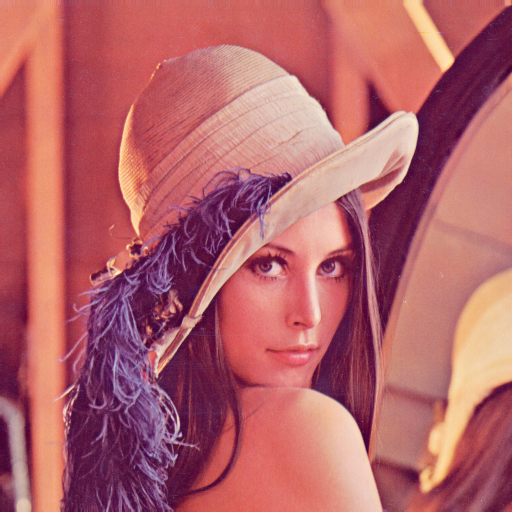
\includegraphics[width=0.5\textwidth]{imagens/Lenna.png}

Fonte: Leader et al. (2003, p. 1228)
\end{figure}

\lipsum[3-56]

\chapter{Primeiro capitulo}

\lipsum[3-56]

% ---
\section{Segundo capitulo}
\chapter{Lectus lobortis condimentum}

% ---
\section{Vestibulum ante ipsum primis in faucibus orci luctus et ultrices
posuere cubilia Curae}
% ---

% ---
% segundo capitulo de Resultados
% ---
\chapter{Nam sed tellus sit amet lectus urna ullamcorper tristique interdum
elementum}

\section{Pellentesque sit amet pede ac sem eleifend consectetuer}


% ---
% Finaliza a parte no bookmark do PDF, para que se inicie o bookmark na raiz
% ---
\bookmarksetup{startatroot}% 
% ---

% ---
% Conclusão
% ---
\chapter*[Conclusão]{Conclusão}
\addcontentsline{toc}{chapter}{Conclusão}

\lipsum[31-33]

% ----------------------------------------------------------
% ELEMENTOS PÓS-TEXTUAIS
% ----------------------------------------------------------
\postextual


% ----------------------------------------------------------
% Referências bibliográficas
% ----------------------------------------------------------
\bibliography{abntex2-modelo-references}


%---------------------------------------------------------------------
% INDICE REMISSIVO
%---------------------------------------------------------------------

\printindex

\end{document}
